%%%%
% Consiglio la visione dei seguenti tutorial:
% - https://www.youtube.com/watch?v=ihxSUsJB_14
% - https://www.youtube.com/watch?v=XTFWaV55uDo
%%%%
\documentclass[12pt,a4paper,openright,twoside]{book}
\usepackage[utf8]{inputenc}
\usepackage{subcaption}
\newcommand{\fonte}[1]{{\color{gray} \small \hypersetup{citecolor=gray} Source: #1}}

%\newcommand{\thesislang}{italian} % decommentare in caso di tesi in italiano
\newcommand{\thesislang}{english} % commentare in caso di tesi in italiano
\usepackage{thesis-style}
% version
\newcommand{\versionmajor}{0}
\newcommand{\versionminor}{1}
\newcommand{\versionpatch}{2}
\newcommand{\version}{\versionmajor.\versionminor.\versionpatch}
\typeout{Document version: \version}

\begin{document}
	
\frontmatter

% ! TeX root = thesis-main.tex
\title{Title}
\author{Candidate Name Here}
\date{\today}

\newgeometry{margin=0.8in}
\begin{titlepage}
	\begin{center}
		% \vspace*{0.2cm}
		
		\large
		\textbf{ALMA MATER STUDIORUM -- UNIVERSITÀ DI BOLOGNA \\ CAMPUS DI CESENA}
		\\
		\noindent\hrulefill
		\vspace{0.4cm}
		
		\Large
		Scuola di Ingegneria e Architettura \\
		Corso di Laurea Magistrale in Ingegneria e Scienze Informatiche
		
		\Huge
		\vspace{4cm}
		\textbf{
			Aggregate Computing and Many-Agent Reinforcement Learning: 
			Towards a Hybrid Approach
		}
		
		\large
		\vspace{1cm}
		Tesi di laurea in 
		\\ 
		\textsc{Pervasive Computing}
		
		\vspace{5.5cm}
		\begin{minipage}[t]{0.64\textwidth}
			\begin{flushleft}
				\textit{Relatore} 
				\\ 
				\textbf{Prof.} \textbf{Mirko Viroli}
				\\
				\vspace{0.4cm}
				\textit{Correlatore} 
				\\
				\textbf{Dott.} \textbf{Gianluca Aguzzi}
			\end{flushleft}
		\end{minipage}
		\begin{minipage}[t]{0.34\textwidth}
			\begin{flushright}
				\textit{Candidato} 
				\\ 
				\textbf{Davide Domini}
			\end{flushright}
		\end{minipage}\\
		
		\vfill
		\noindent\hrulefill
		\vspace{0.3cm}
		\Large
		
		Seconda Sessione di Laurea
		\\
		Anno Accademico 2022-2023
	\end{center}
\end{titlepage}
\restoregeometry


\begin{abstract}	
Max 2000 characters, strict.
\end{abstract}

\begin{dedication} 
Optional. Max a few lines.
\end{dedication}

\begin{acknowledgements}
Optional. Max 1 page.
\end{acknowledgements}

%----------------------------------------------------------------------------------------
\tableofcontents   
\listoffigures     
\lstlistoflistings 
%----------------------------------------------------------------------------------------

\mainmatter

%----------------------------------------------------------------------------------------
\chapter{\introductionname}
\label{chap:introduction}
%----------------------------------------------------------------------------------------


\paragraph{Thesis motivation} % TODO --- Riformulare e approfondire meglio

Significant technological advancements have paved the way for the emergence of a field known as \emph{Collective Computing} 
    \cite{abowd2016beyond}, with \emph{Cyber-Physical Swarms (CPSW)} \cite{schranz2021swarm} as a noteworthy branch within it.
    The latter consist of myriad devices that interact with the environment and exchange information among themselves. 
    A crucial aspect of these systems is that a more complex collective behavior emerges from the interaction between 
    individual agents that leads to the resolution of various tasks.
    Among all aspects related to CPSW, our focus lies on properties like \emph{collective intelligence} \cite{tumer2004survey} 
    and \emph{self-organization} \cite{schmeck2011organic}. This stems from the applications of these systems, leading us to 
    concentrate on their collective behavior to express autonomy, adaptability, and coordination of the devices 
    that are part of them.

This progress has been driven by research in various related fields such as: multi-agent systems \cite{dorri2018multi},
     coordination \cite{yang2022overview}, distributed artificial intelligence \cite{bond2014readings}, and many others. 
     Additionally, it has a profound impact on a wide range of applied domains, including: smart cities \cite{zedadra2019swarm}, 
     swarm robotics \cite{brambilla2013swarm}, large-scale IoT systems \cite{uslu2023role}, and more.

A crucial aspect to consider in CPSW is how individual devices are programmed and achieve coordination to perform assigned tasks. 
Novel approaches -- like \emph{aggregate computing} \cite{viroli2018field} -- have focused on manually developing
controllers from a global perspective. However, this approach has some drawbacks: it is highly challenging to write satisfactory 
and efficient programs for complex tasks, they may be error-prone and lack of generality.

On the other hand, there exists approaches that leverage various artificial intelligence (AI) techniques, 
such as \emph{Multi-Agent Reinforcement Learning} (MARL) \cite{busoniu2008comprehensive},
to enable devices to learn directly from experience and/or data. These approaches also present several challenges, including: non-stationarity 
\cite{hernandez2017survey}, communication and scalability.

%
\paragraph{Thesis objectives}

Starting from what was seen in the previous paragraph, the goal of this thesis is to lay the foundation for a hybrid approach 
    that can succeed in exploiting the potential of both macro-programming, in particular \emph{aggregate computing} is taken as a 
    reference, and AI approach.
    In order to achieve this goal, it is necessary to develop a toolchain that allows these systems to be developed in an agile,
    fast and reusable way. 
    Scarlib, whose development has already started in \cite{scarlib}, is the tool that for us forms the basis of this toolchain.
    Its main purpose is to integrate the \emph{ScaFi} \cite{casadei2022scafi} (an implementation of aggregate computing) 
    and \emph{Alchemist} \cite{pianini2013chemical} (a bio-chemical based simulator) tools with \emph{Reinforcement Learning} 
    to help develop experiments in \emph{simulated} environments with \emph{offline learning}.

%
\paragraph{Thesis Structure} 


%----------------------------------------------------------------------------------------
\chapter{Background}
\label{chap:background}
%----------------------------------------------------------------------------------------

\section{Cyber-Physical Swarms}
%
\section{Aggregate Computing}

The advent of \emph{Collective Computing} and the proliferation of interconnected devices have given rise to novel 
    paradigms that aim to address the challenges posed by the distributed nature of computing
    systems. One such paradigm that has gained significant attention in recent years is 
    \emph{aggregate computing (AC)} [8].

AC is well grounded on \emph{field calculus}, and therefore adopts a model where the perspective is at a global level: 
    a group of devices is seen as a global entity (i.e., the \emph{aggregate system}) that works at asynchronous 
    rounds and exchanges messages with neighbours. 
    A round is composed of three phases:
    i) \emph{Context Building}, each node collects information from the 
        neighborhood and sensors,
    ii) \emph{Program Execution}, each node executes the aggregate program on the local context, and
    iii) \emph{Export Sharing}, each node shares the export with the neighborhood.

Interactions within the aggregate system are seen as a flow of information propagating through the 
    collective of devices, rather than as local interactions of individual devices with their
    peers and the environment. This approach offers a number of advantages:
    i) the program can be defined in a composable and declarative manner, 
    ii) it promotes the reuse of behaviours, and 
    iii) the programmer is relieved from concerns regarding low-level aspects (e.g., failures, distribution, communication and more), 
    as these are automatically handled by the middleware.
%Considering the interactions within this system as a flow of information 
%    propagating through a collective of devices, rather than as local interactions between devices and the 
%    environment, offers significant advantages: i) the program can be defined in a composable and declarative
%    manner, ii) it promotes the reuse of behaviours, and iii) the programmer is relieved from concerns regarding 
%    low-level aspects (e.g., failures, distribution, communication and more), as these are automatically handled 
%    by the middleware. %riformula tipo "le interazioni sono viste come... e questo porta i seguenti vantaggi..."

In aggregate computing, information is represented by a distributed data structure known as computational field [50, 26],
    which is an abstraction of space-time values where each device is mapped to a computational value.
    The manipulation of these fields is derived from the Field Calculus [48], a computational model in which collective 
    behaviours are expressed as algorithms that are the composition of computational fields.

In recent times, several implementations of aggregate computing have been developed, and one particularly interesting 
    implementation is ScaFi [13]. ScaFi is a Scala-based platform that offers the following features: 
    i) a domain specific language (DSL) for specifying aggregate computation, 
    ii) asimulation environment (through the Alchemist simulator [34]), 
    iii) a middleware for executing and deploying aggregate programs, and 
    iv) reusable library functionalities that serve as building blocks for constructing new aggregate programs. 
    For example, the gradients abstraction that provides gradient functions [47, 7] used for the ongoing computation, 
    across spatio-temporal dimension, of the self-healing field (i.e., a field able to self-adjust in case of changes 
    in devices topology) that determines the minimum distances of individual nodes from a specified set of source 
    nodes [13].

\begin{figure}[h!]
    \centering
    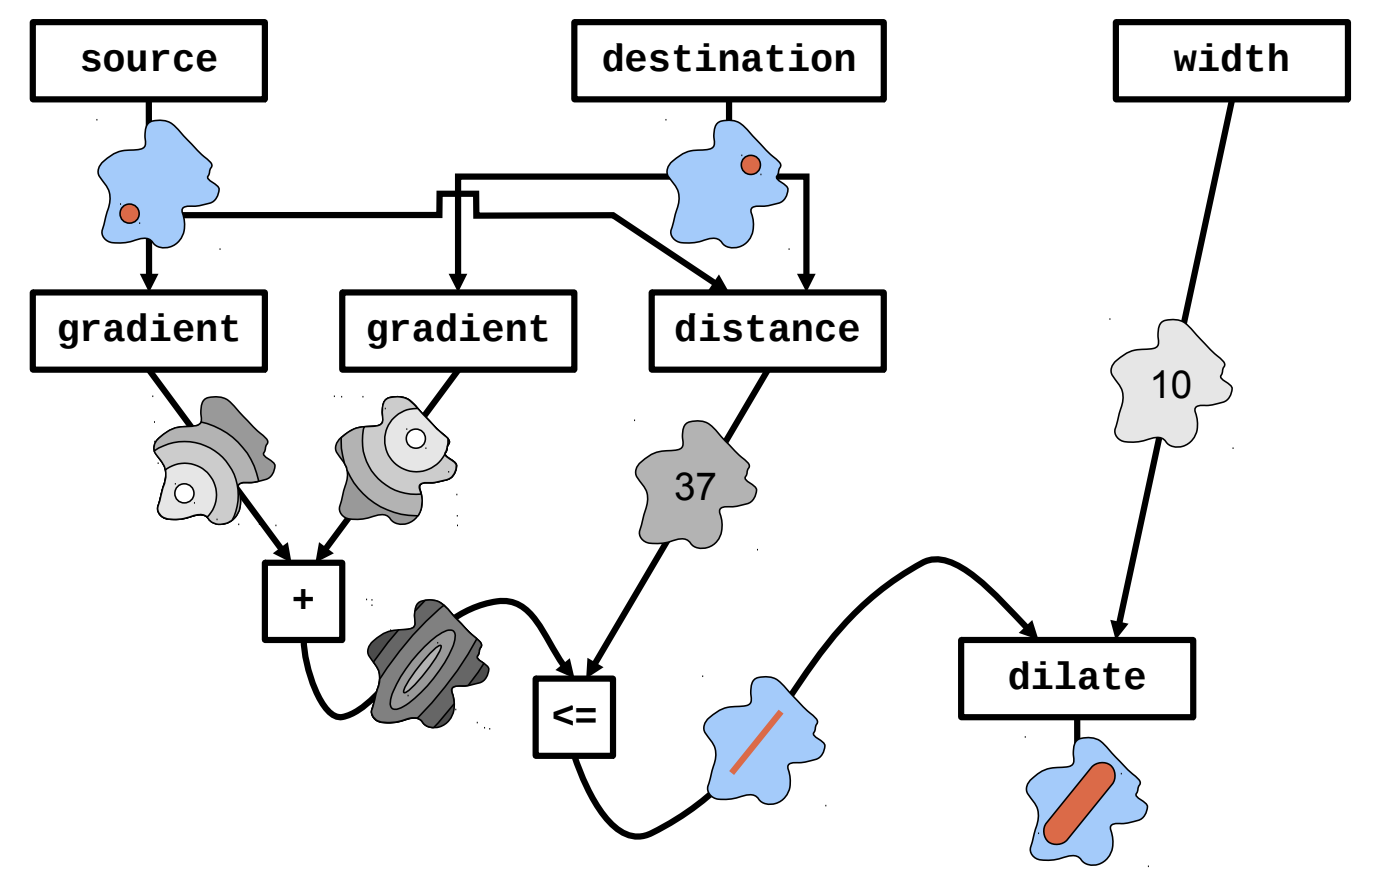
\includegraphics[width=0.7\textwidth]{figures/channel.png}
    \caption{Channel example}
    \label{fig:channel}
\end{figure}

\lstinputlisting[float,language=Scala,label={lst:channel-code}]{listings/Channel.scala}

%
\section{Reinforcement Learning}
%

``\emph{Reinforcement Learning (RL)} is the science of decision making. It is about learning the optimal behavior 
    in a environment to obtain maximum reward" 
    \footnote{\url{https://www.synopsys.com/ai/what-is-reinforcement-learning.html}}.
    RL is a general framework, other than supervised and unsupervised learning, in which an \emph{agent} learns 
    to behave within an \emph{environment} by performing some \emph{actions} and seeing the result they produce.
    It is inspired by how humans and animals learn through the system of rewards and punishments: for each good action
    the environment provides to the agent a positive reward, instead, for each bad action the agent gets a negative 
    reward (also called penalty).

Formally, a RL problem can be formulated as following \cite{RLSurvey}:
    \begin{itemize}
        \item Discrete time steps $t=0, 1, 2, ...$;
        \item A discrete set of environment states $\mathcal{S}$;
        \item A discrete set of agent actions $\mathcal{A}$;
        \item A reinforcement signal;
        \item A probabilistic policy $\pi$, that is a mapping function from states to actions;
        \item The goal of the agent is to learn the optimal policy $\pi^*$ in order to maximize 
                some long-run measure of reinforcement (e.g., the Infinite Horizon Discounted Model \cite{RLSurvey}).
    \end{itemize}
    First, at time $t$, the agent observes the state of the environment $s_t \in \mathcal{S}$
        and chooses an action $a_t \in \mathcal{A}$ using the actual policy $\pi_t$. 
        Thereafter, the environment: takes in the action $a_t$, emits the new state $s_{t+1} \in \mathcal{S}$ 
        and returns the scalar reward $r_{t+1}$ (\Cref{fig:rl_schema}).
        Finally, the agent, based on the reward obtained updates its knwoledge.
    This formulation stems from \emph{Markov Decision Processes}, which is a mathematical framework for \emph{sequential decision making}. A very important property that these systems must adhere to is the \emph{Markov property}, which states ``\emph{the future is independent of the past given the present.}" In other words, it implies that the state transition function does not require the entire past trajectory but only the last state, namely: 
    $$p(s_{t+1} | s_t, a_t, ..., s_0, a_0) = p(s_{t+1} | s_t, a_t)$$
    It is important to note that the concept of state can always be extended to satisfy this property.


\begin{figure}[t]
    \centering
    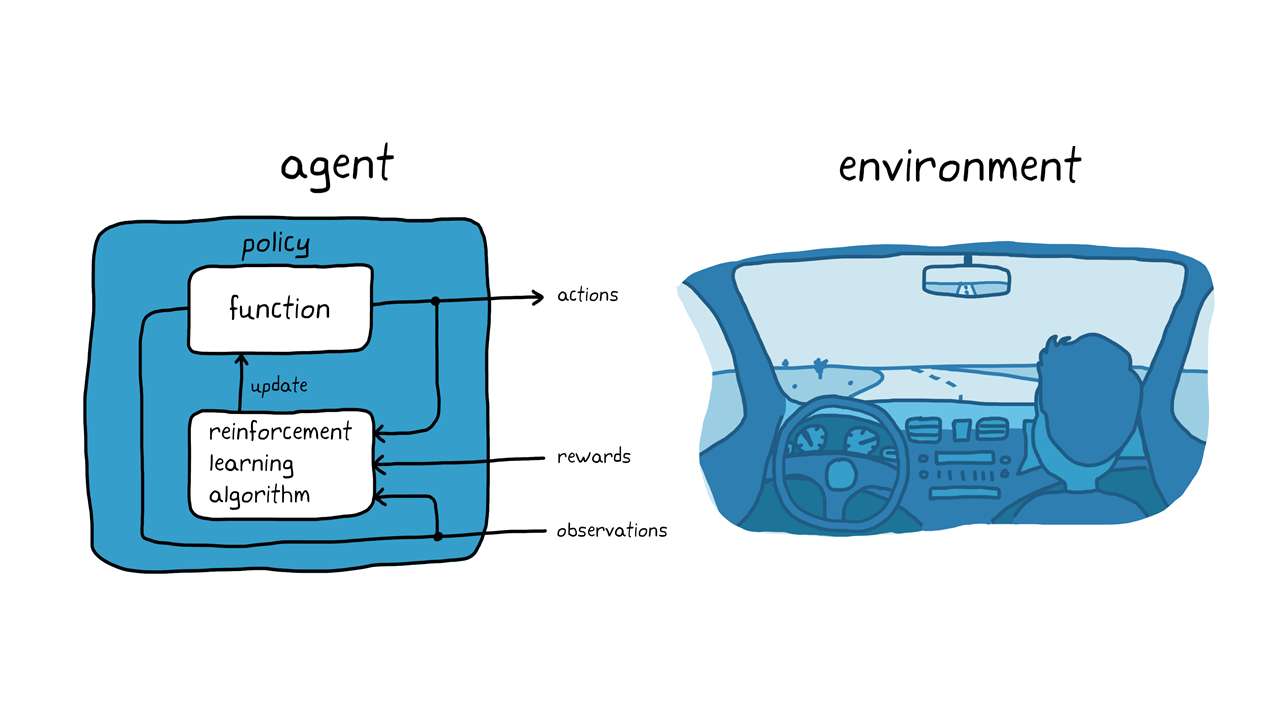
\includegraphics[width=0.7\textwidth]{figures/rl.png}
    \caption{Agent-environment interactions}
    \fonte{\url{https://it.mathworks.com/discovery/reinforcement-learning.html}}
    \label{fig:rl_schema}
\end{figure}

In order to find the optimal policy $\pi^*$, the agent tries to maximize the expected cumulative reward.
    Since the environment is stochastic (i.e., the same action performed in the same state could lead to different 
    results over time) the more you look into the future the more the outcome could diverge.
    For this reason, it is common to use a model that takes less account of rewards that are far away in time 
    than those that are close in time:
    $$R_t = \sum_{i=t}^{\infty} \gamma^{i-t} \cdot R_{\pi(s_i)}(s_i, s_{i+1}) $$
    This model is called \emph{Infinite Horizon Discounted Model}, the key aspect is the hyper-parameter $\gamma$.
    It is a scalar weight in the range $[0;1]$, in this way, the further away the reward is in time, the smaller its weight.

\paragraph{Exploration-exploitation dilemma}

The \emph{exploration-exploitation dilemma} is a problem that comes from the definition of the RL process.
    In order to increase its knowledge and build an optimal policy, the agent needs to \emph{explore} the environment 
    in the hope of finding better actions. After some exploration, the agent might have found a set of 
    apparently rewarding actions, but, how can the agent be sure that the found actions are actually the best? 
    When should the agent continue to explore or else, when should it just \emph{exploit} its existing knwoledge?

Several exploration strategies have been proposed in the literature to solve this problem, the simplest is the
    \emph{$\epsilon$-greedy} strategy. The agent \emph{randomly explore} the environment with probability $\epsilon$
    while \emph{exploit} the current optimal action with probability $1-\epsilon$.

    $$
    \pi(s)=
    \begin{cases}
        \pi^*(s) & \text{with probability $1-\epsilon$} \\
        \text{\emph{random action}} & \text{with probability $\epsilon$}\\
    \end{cases} 
    $$ 

    Usually, at the beginning of the learning process $\epsilon$ starts near to $1$ (i.e., more exploration) and then decreases
    to $0$ as the agent learns more and more about the environment. 

\paragraph{Main approaches}

In Reinforcement Learning, there are two main families of approaches that can be used to categorize the 
    algorithms employed by an agent in finding the optimal policy. These are: 
    i) policy-based methods, and 
    ii) value-based methods.
    Policy-based algorithms aim to directly learn a function that maps each state to the best action to take 
    (or a probability distribution over a set of possible actions). On the other hand, value-based methods 
    seek to learn a function that maps each possible state to an expected value of being in that state. 
    This way, the agent can learn which states is more valuable and will take action that leads to it. 
    This comparison is well illustrated in \Cref{fig:rl-methods}.

An example of policy-based method is \emph{Proximal Policy Optimization (PPO)} \cite{ppo}, while an example of 
    value based-method is \emph{Q-Learning} \cite{QL}

\begin{figure*}[t]
    \begin{subfigure}[b]{0.49\textwidth}
        \centering
        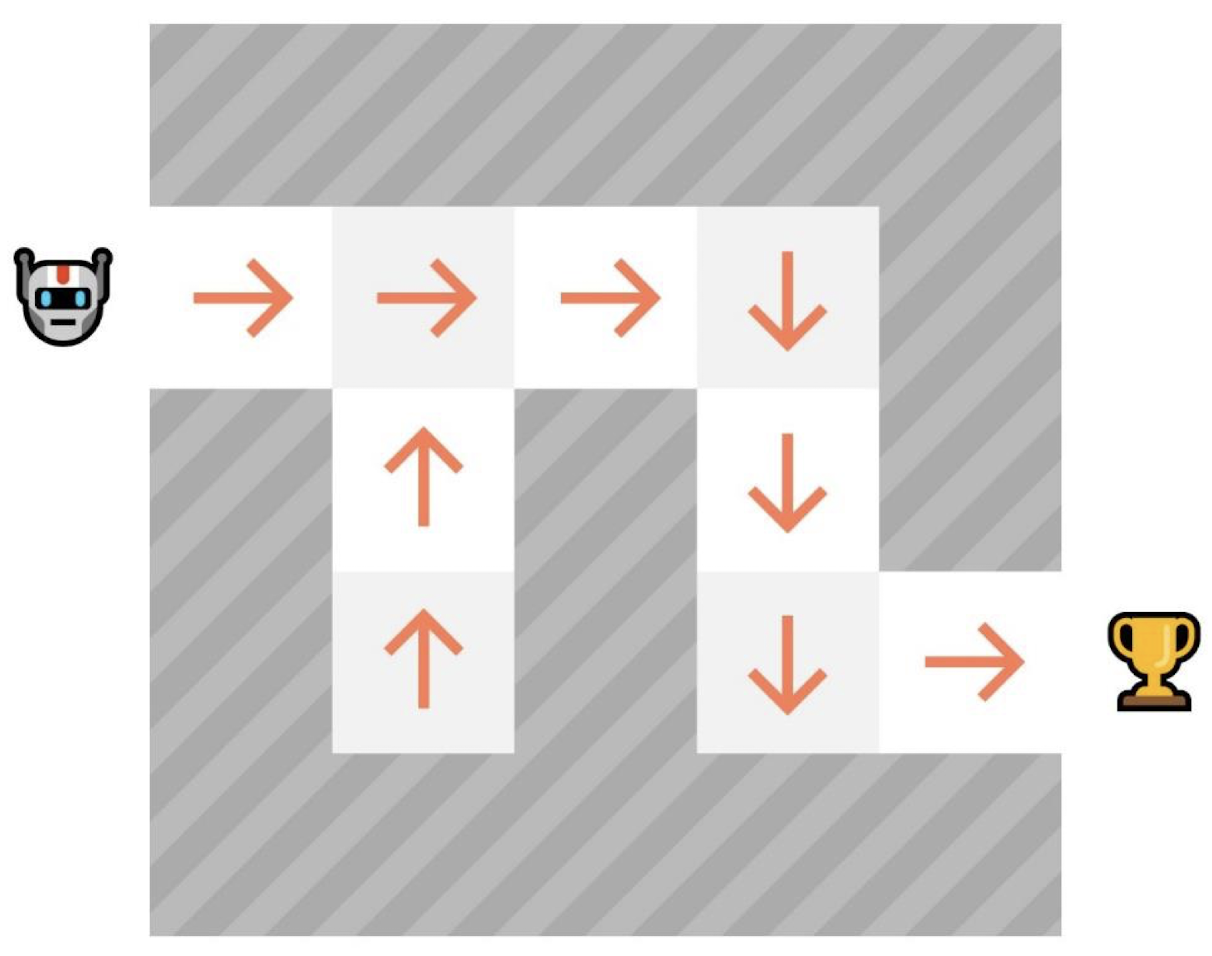
\includegraphics[width=0.7\textwidth]{figures/policy-based-rl.png}
        \caption{Policy based RL}
        \label{fig:policy-based-rl}
    \end{subfigure}
    \begin{subfigure}[b]{0.49\textwidth}
        \centering
        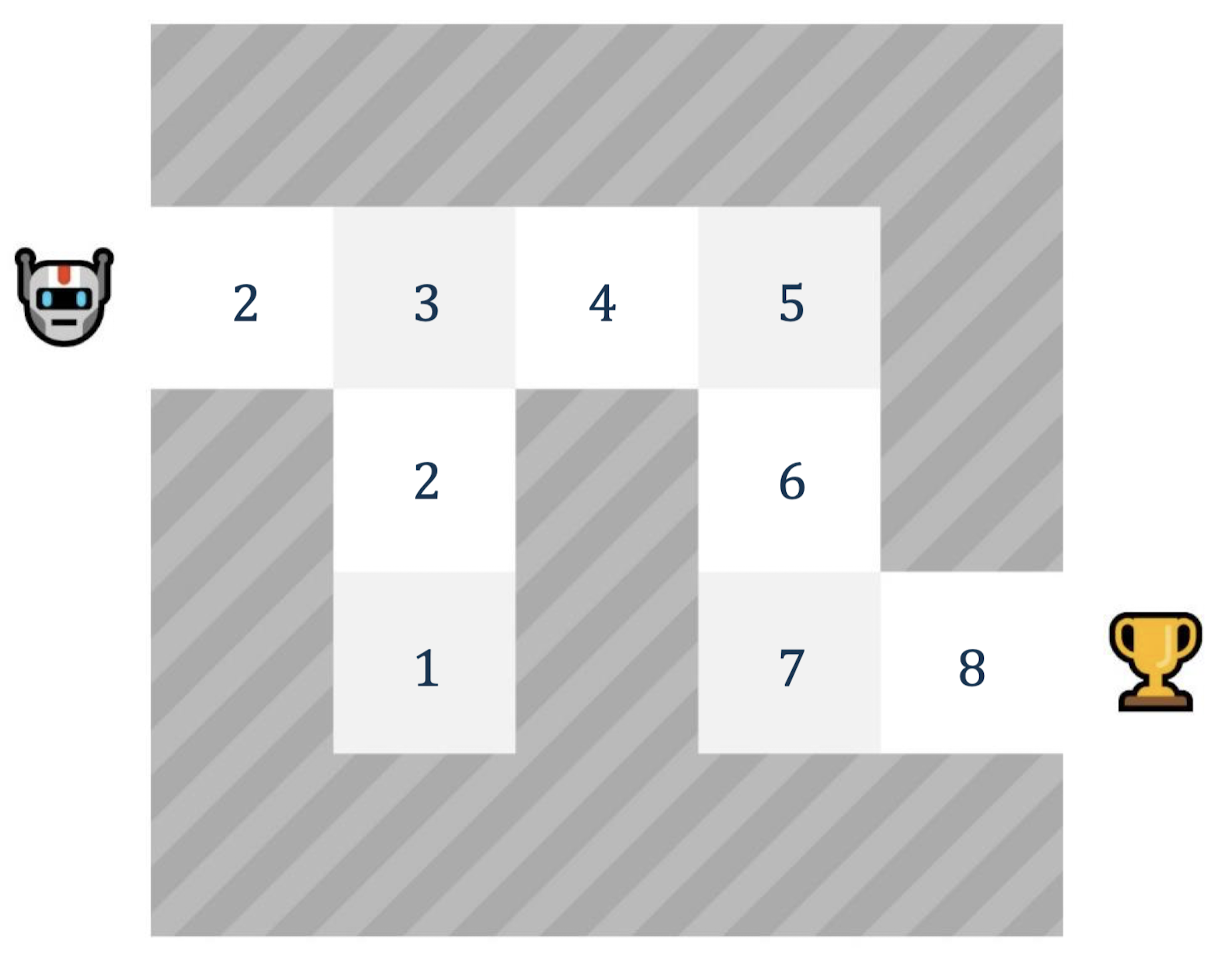
\includegraphics[width=0.7\textwidth]{figures/value-based-rl.png}
        \caption{Value based RL}
        \label{fig:value-based-rl}
    \end{subfigure}
\caption{Policy and value based algorithms visual comparison}%\vspace{-10pt}
\fonte{\url{https://www.lamsalashish.com.np/blog/reinforcement-learning}}
\label{fig:rl-methods}
\end{figure*}

\paragraph{Q-Learning}

\emph{Q-Learning} is one of the most famous Reinforcement Learning algorithms from the value-based methods family. 
    One of the key aspects of this algorithm is the \emph{Q-Table}, denoted as $Q(s,a)$. This table represents, 
    for each possible state-action pair, the \emph{expected cumulative reward} that the agent will obtain by
    taking action $a$ in state $s$ and subsequently following optimal actions. 
    Thus, the Q-table at time step $t$, given a state $s_t$, an action $a_t$, and a policy $\pi_t$, is represented by:
    $$ Q(s_t, a_t) = max_{\pi(s_t) = a_t} R_{t+1}$$
    Starting from the Q-Table, one can easily define the \emph{optimal policy} as follows:
    $$ \pi^{*}(s) = argmax_a Q(s,a) $$

Another key aspect is how we can estimate the reward at the end of the process if we only know the current state 
    and action, without knowing the subsequent trajectory. To achieve this, the \emph{Bellman equation} can be used. 
    This equation defines, for a given transition $<s_t, a_t, s_{t+1}, r_{t+1}>$, the value $Q(s,a)$ recursively 
    as the sum of the immediate reward and the maximum expected cumulative reward from the subsequent state:
    $$ Q(s_t,a_t) =  r_{t+1} + \gamma \cdot max_a Q(s_{t+1}, a)$$

The main idea of Q-Learning is to \emph{iteratively approximate} the Q-values, using the Bellman equation, as follows:
$$ Q^{new}(s_t,a_t) = (1-\alpha) \cdot Q(s_t,a_t) + \alpha \cdot (r_{t+1} + \gamma \cdot max_a Q(s_{t+1}, a)) $$
    Where $\alpha$ is the learning rate hyper-parameter that controls how much of the current Q-value and newly proposed
    Q-value is considered.
    At the beginning of the learning process, these Q-values will be practically random estimates and may be completely wrong. 
    However, it has been demonstrated that as iterations progress, these Q-values will 
    converge and represent the true Q-values.

\paragraph{Deep Reinforcement Learning}

Classical algorithms of reinforcement learning, when applied in \emph{real-world contexts}, suffer from the problem of \emph{state space explosion}.
    This arises from an exceedingly large number of possible states, making the resolution of a given task \emph{computationally intractable}. 
    For instance, in the game of chess, there can be around $100^{100k}$ possible games, a number much larger than 
    the count of sand grains on Earth ($\approx 10^{23}$) and the number of atoms in the observable universe 
    ($\approx 10^{81}$). 
    For this reason, \emph{deep reinforcement learning} has been introduced, which involves utilizing deep neural networks
    as approximators for the policy and/or the value function.

One of the most well-known Deep RL algorithms is DQN \cite{dqn}. This was developed by DeepMind in 2013 and was initially
    used to train an agent capable of playing Atari video games. One of the advantages of using neural networks as 
    approximators for the function to be learned is the ability to avoid hand-engineering the state space and instead 
    allow the network to learn the best features directly. For example, in the case of Atari games, this is achieved 
    by using convolutional layers and feeding the network with screen raw pixels.
    
DQN, specifically, is the deep version of the Q-Learning algorithm, thus producing a Q-Value output for each 
    possible action (\Cref{fig:qlvsdqn}). This makes the training of the utilized neural network a regression task 
    in which a squared error loss can be employed as the loss function:
    $$ L = (y_t - \hat{y_t})^2 $$
    Where $y_t$ represents the actual value and $\hat{y_t}$ is the predicted value at time t. Since RL is an 
    unsupervised learning, and therefore labels are not available, the value $y_t$ is estimated using the 
    Bellman equation, transforming the loss function for a transition $<s_t, a_t, s_{t+1}, r_{t+1}>$ into:
    $$ L = ( r_{t+1} + \gamma \cdot max_a Q(s_{t+1}, a) - Q(s_t, a_t))^2 $$

\begin{figure*}[t]
    \begin{subfigure}[b]{0.49\textwidth}
        \centering
        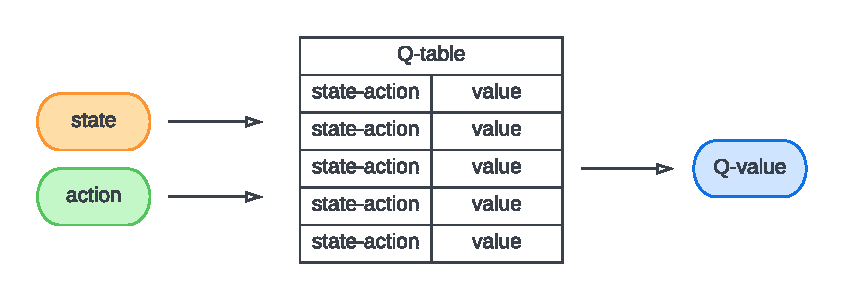
\includegraphics[width=\textwidth]{figures/q-learning.pdf}
        \caption{Q-Learning}
        \label{fig:ql}
    \end{subfigure}
    \begin{subfigure}[b]{0.49\textwidth}
        \centering
        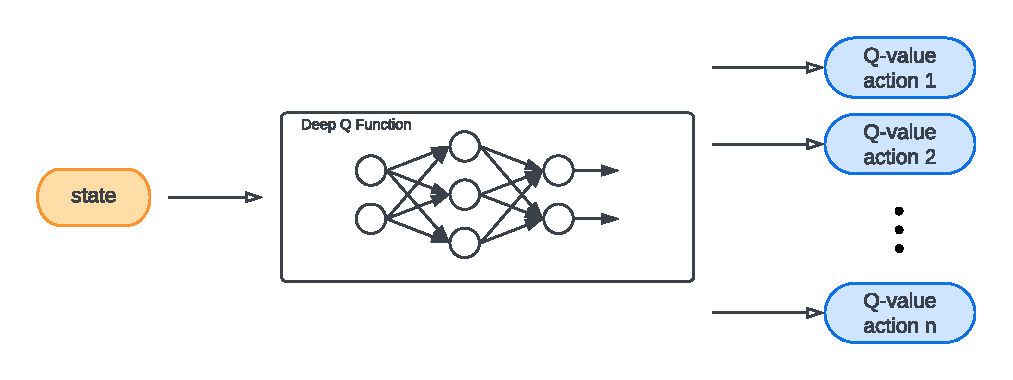
\includegraphics[width=\textwidth]{figures/deepQL.pdf}
        \caption{Deep Q-Learning}
        \label{fig:dqn}
    \end{subfigure}
\caption{Q-Learning and Deep Q-Learning visual comparison}\vspace{-10pt}
\label{fig:qlvsdqn}
\end{figure*}

When attempting to use neural networks to approximate the Q-function, several problems arise. 
    The first one is due to the high correlation that exists between two consecutive transitions within the same 
    episode. This correlation leads to a significant decrease in variance, causing the network to tend to forget 
    previous transitions as it overwrites them with newer ones. For instance, let's consider an agent's task to 
    learn to play a level-based video game; this issue implies that while the agent tries to learn how to navigate 
    the second level, it might forget how to behave in the first level. The most common solution is to employ an 
    \emph{experience replay} (i.e., a buffer), where all transitions $<s_t, a_t, s_{t+1}, r_{t+1}>$ are stored. 
    When updating weights, a random mini-batch is sampled from this buffer, breaking the correlation between consecutive
    transitions. Furthermore, since a transition can be used in multiple weight updates, this approach also 
    improves data efficiency.

A second issue that can be observed is referred to as the \emph{moving target problem}. This stems from the fact that,
    when updating the network's weights, both the predicted values and the target values are estimated using the 
    same neural network. This leads to a strong correlation between the target values and the network's weights, 
    introducing significant oscillations during training. To address this problem, two distinct neural networks 
    with identical architecture are employed: 
    i) \emph{the action network $Q$}, used to determine the agent's actions, which is updated every $u$ steps; 
    ii) \emph{the target network $\hat{Q}$}, used to calculate the target values, updated every $c$ steps. 
    Typically, $c >> u$, and the \emph{target network's} weight update involves replacing the existing weights with 
    those from the \emph{action network}.
    Since the target values are generated using an older set of weights, a delay is introduced between the 
    moment the $Q$ network is updated and the moment it starts to affects the target values.
    This delay reduces the likelihood of divergence and oscillations. The loss function becomes:
    $$ L = ( r_{t+1} + \gamma \cdot max_a \hat{Q}(s_{t+1}, a) - Q(s_t, a_t))^2 $$

\section{Multi-Agent Reinforcement Learning}

%----------------------------------------------------------------------------------------
\chapter{Requirements} 
\label{chap:requirements}
%----------------------------------------------------------------------------------------


%----------------------------------------------------------------------------------------
\chapter{Design} 
\label{chap:design}
%----------------------------------------------------------------------------------------


%----------------------------------------------------------------------------------------
\chapter{Implementation} 
\label{chap:implementation}
%----------------------------------------------------------------------------------------


%----------------------------------------------------------------------------------------
\chapter{Validation} % possible chapter for Projects
\label{chap:validation}
%----------------------------------------------------------------------------------------


%----------------------------------------------------------------------------------------
\chapter{\conclusionsname}
\label{chap:conclusions}
%----------------------------------------------------------------------------------------


%----------------------------------------------------------------------------------------
% BIBLIOGRAPHY
%----------------------------------------------------------------------------------------

%\nocite{*} % uncomment this to show all the reference in the .bib file
\bibliographystyle{plain}
\bibliography{bibliography}


\end{document}